% !TEX TS-program = pdflatex
\documentclass[aspectratio=169]{beamer}
\usepackage[utf8]{inputenc}
\usepackage[T1]{fontenc}
\usetheme{Madrid}
\usecolortheme{seahorse}
\usefonttheme{professionalfonts}
\setbeamertemplate{navigation symbols}{}
\setbeamercovered{transparent}
\setbeamertemplate{itemize items}[circle]
\setbeamertemplate{enumerate items}[default]
\setlength{\parskip}{0.15em}

\definecolor{bepurple}{RGB}{107,63,160}
\definecolor{begold}{RGB}{200,168,75}
\definecolor{beteal}{RGB}{26,122,110}
\definecolor{berust}{RGB}{192,68,42}
\definecolor{beblue}{RGB}{26,74,138}
\definecolor{softpurple}{RGB}{240,232,255}
\definecolor{softgold}{RGB}{255,248,220}
\definecolor{softteal}{RGB}{220,242,240}
\definecolor{softrust}{RGB}{255,235,230}
\setbeamercolor{structure}{fg=beblue}
\setbeamercolor{title}{fg=white,bg=beblue}
\setbeamercolor{frametitle}{fg=beblue}
% Minimal block rendering: regular/example blocks become colored headings (no box)
\setbeamertemplate{block begin}{%
  \par\vspace{0.2ex}%
  \ifx\insertblocktitle\empty\else%
    {\usebeamerfont{block title}\color{beblue}\textbf{\insertblocktitle}}\par\vspace{0.2ex}%
  \fi%
}
\setbeamertemplate{block end}{\par\vspace{0.2ex}}
\setbeamertemplate{block example begin}{%
  \par\vspace{0.2ex}%
  \ifx\insertblocktitle\empty\else%
    {\usebeamerfont{block title}\color{beteal}\textbf{\insertblocktitle}}\par\vspace{0.2ex}%
  \fi%
}
\setbeamertemplate{block example end}{\par\vspace{0.2ex}}
\setbeamertemplate{block alerted begin}{%
  \par\vspace{0.5ex}%
  \begin{beamercolorbox}[sep=0.5ex,rounded=true,shadow=false]{block title alerted}%
    \usebeamerfont{block title}\insertblocktitle%
  \end{beamercolorbox}%
  \nointerlineskip%
  \begin{beamercolorbox}[sep=0.5ex,rounded=true,shadow=false]{block body alerted}%
    \usebeamerfont{block body}%
}
\setbeamertemplate{block alerted end}{\end{beamercolorbox}\par\vspace{0.5ex}}
\setbeamercolor{block title alerted}{fg=white,bg=berust}
\setbeamercolor{block body alerted}{fg=black,bg=berust!8}
\setbeamercolor{alerted text}{fg=berust}

\usepackage{booktabs,amsmath,amssymb,array,multirow,hyperref,colortbl,xcolor}
\usepackage{tikz}
\usepackage{pgfplots}
\pgfplotsset{compat=1.18}
\usetikzlibrary{arrows.meta,positioning,calc,shapes.geometric,patterns}
\hypersetup{colorlinks=true,linkcolor=beblue,urlcolor=beblue}

\title{\textbf{Lecture 3: Prospect Theory}}
\subtitle{Decision Under Risk --- Beyond Expected Utility}
\author{Prof.\ Muhebullah Karimzada}
\institute{School of Economics, University of Northern British Columbia}
\date{ECON 230 $\cdot$ Introduction to Behavioural Economics $\cdot$ Winter 2027}

\begin{document}

\begin{frame}[plain]\titlepage\end{frame}

% ============================================================
\begin{frame}{Opening Game --- Your Risk Preferences}
\note{Run all three problems before any discussion. Collect hands. The pattern --- risk averse in gains, risk seeking in losses --- is what prospect theory explains.}
\begin{alertblock}{Make your choices --- write them down}
\textbf{Problem 1:} A) Win \$900 for certain. \quad B) 90\% chance of \$1,000, 10\% chance of \$0.\\[0.4em]
\textbf{Problem 2:} A) Lose \$900 for certain. \quad B) 90\% chance of losing \$1,000, 10\% chance of losing \$0.\\[0.4em]
\textbf{Problem 3:} You have \$2,000. \quad A) Lose \$500 for certain. \quad B) 50\% chance of losing \$1,000.
\end{alertblock}
\pause
\begin{block}{Typical Results}
\begin{itemize}
  \item Problem 1: \textbf{84\% choose A} --- risk averse in \textit{gains}
  \item Problem 2: \textbf{87\% choose B} --- risk \textit{seeking} in \textit{losses}
  \item Problem 3: \textbf{69\% choose B} --- frame as loss $\Rightarrow$ gamble to avoid certain loss
\end{itemize}
\textcolor{bepurple}{\textbf{EU cannot explain this pattern. Prospect Theory can.}}
\end{block}
\end{frame}

% ============================================================
\begin{frame}{Lecture Roadmap}
\begin{enumerate}[<+->]
  \item Why EU fails --- the four-fold pattern
  \item \textbf{Reference dependence} --- gains and losses, not final wealth
  \item \textbf{Loss aversion} --- $\lambda \approx 2.25$
  \item \textbf{The S-shaped value function} --- THE key diagram
  \item \textbf{Probability weighting} --- the inverse-S function
  \item Cumulative Prospect Theory (Tversky \& Kahneman, 1992)
  \item Applications: disposition effect, endowment effect, insurance, housing, health
\end{enumerate}
\end{frame}

% ============================================================
\section{Why Expected Utility Fails}
% ============================================================

\begin{frame}{The Four-Fold Pattern}
\begin{center}
\begin{tabular}{p{3cm}p{4.5cm}p{4.5cm}}
\toprule
 & \textbf{Gains} & \textbf{Losses}\\
\midrule
\textbf{High Probability} & \cellcolor{softteal} \textbf{Risk Averse} \newline Prefer certain gain \newline \textit{``Lock in the win''} & \cellcolor{softrust} \textbf{Risk Seeking} \newline Gamble to avoid certain loss \newline \textit{``Roll the dice''}\\[1em]
\textbf{Low Probability} & \cellcolor{softrust} \textbf{Risk Seeking} \newline Buy lottery tickets \newline \textit{``Dream big''} & \cellcolor{softteal} \textbf{Risk Averse} \newline Buy insurance \newline \textit{``Protect against disaster''}\\
\bottomrule
\end{tabular}
\end{center}
\medskip
\begin{exampleblock}{EU Prediction}
With a concave utility function, EU predicts \textit{always} risk averse --- for all probabilities and gains/losses. The four-fold pattern is a systematic empirical refutation.
\end{exampleblock}
\end{frame}

% ============================================================
\begin{frame}{Framing Effects Cannot Be Explained by EU}
\begin{block}{The Asian Disease Problem (Kahneman \& Tversky, 1981)}
A disease threatens 600 lives. Two programmes available:
\end{block}
\begin{columns}
\column{0.48\textwidth}
\begin{block}{Gain Frame}
\begin{itemize}
  \item A: 200 people saved
  \item B: 1/3 prob 600 saved, 2/3 prob 0 saved
\end{itemize}
\textcolor{beteal}{\textbf{72\% choose A (safe option)}}
\end{block}
\column{0.48\textwidth}
\begin{alertblock}{Loss Frame}
\begin{itemize}
  \item C: 400 people die
  \item D: 1/3 prob 0 die, 2/3 prob 600 die
\end{itemize}
\textcolor{berust}{\textbf{78\% choose D (risky option)}}
\end{alertblock}
\end{columns}
\medskip
\begin{alertblock}{A = C and B = D. EU Cannot Explain This.}
Under EU, utility is over final outcomes (lives saved). Describing the same outcome as ``lives saved'' vs ``deaths'' should not matter. But it does --- dramatically. We need a theory with a \alert{reference point}.
\end{alertblock}
\end{frame}

% ============================================================
\section{Reference Dependence}
% ============================================================

\begin{frame}{The Reference Point}
\begin{block}{Core Idea of Prospect Theory}
People evaluate outcomes as \alert{gains or losses} relative to a \textbf{reference point}, not as levels of final wealth. The same final wealth can be a gain or a loss depending on the reference.
\end{block}
\begin{columns}
\column{0.5\textwidth}
\begin{exampleblock}{What Determines the Reference Point?}
\begin{itemize}
  \item \textbf{Status quo:} Current situation (most common)
  \item \textbf{Expectations:} What you expected to happen
  \item \textbf{Social comparison:} What peers received
  \item \textbf{Budget/target:} What you planned to spend
\end{itemize}
\end{exampleblock}
\column{0.47\textwidth}
\begin{alertblock}{Reference Point Malleability}
Getting a \$500 raise feels like:
\begin{itemize}
  \item A \textbf{GAIN} if you expected \$500
  \item A \textbf{LOSS} if you expected \$1,000
\end{itemize}
Marketers exploit this: ``Compare at \$200 --- our price: \$150.'' The \$200 is the reference point, making \$150 feel like a \$50 gain.
\end{alertblock}
\end{columns}
\end{frame}

% ============================================================
\begin{frame}{Reference Points in Labour Markets}
\begin{block}{Nominal Wage Rigidity (Akerlof, Dickens \& Perry, 1996)}
Workers resist \textbf{nominal wage cuts} even when real wages are falling due to inflation. A 2\% nominal raise with 5\% inflation ($-$3\% real) is \textit{accepted}. A 3\% nominal cut with 0\% inflation ($-$3\% real) is \textit{resisted}. The reference point is the \textit{nominal} wage --- not the real value.
\end{block}
\begin{exampleblock}{Shafir, Diamond \& Tversky (1997)}
Workers preferred a \textbf{5\% raise} (with 12\% inflation = $-$7\% real) over a \textbf{2\% raise} (with 4\% inflation = $-$2\% real). The preferred scenario left them \textit{worse off in real terms} --- because they evaluated the nominal gain, not the real outcome.
\end{exampleblock}
\begin{alertblock}{Canadian Wage Data}
During the 1970s inflation spike (1974--1980, average 9\%), Canadian nominal wages rose 10--12\% annually --- preserving the \textit{perception} of real gains while real wages stagnated.
\end{alertblock}
\end{frame}

% ============================================================
\begin{frame}{Loss Aversion --- The Central Finding}
\note{This single parameter --- lambda approximately 2.25 --- has enormous implications. It explains the equity premium puzzle, disposition effect, contract design, wage rigidity, and much more.}
\textcolor{beblue}{\textbf{Tversky \& Kahneman (1992):}} $\lambda \approx 2.25$ --- losses loom 2.25$\times$ larger than equivalent gains.
\begin{columns}
\column{0.5\textwidth}
\begin{itemize}[<+->]\small
  \item 50/50 bet --- win \$X or lose \$100: most require $X > \$200$.
  \item Butter consumer panel: $\lambda \approx 2.4$ (Hardie et al., 1993).
  \item Capuchin monkeys show loss aversion! (Chen et al., 2009).
  \item Workers accept lower wages when risk framed as bonuses vs penalties (Fryer et al., 2012).
\end{itemize}
\column{0.47\textwidth}
\textcolor{beteal}{\textbf{Operates in:}} stock markets (disposition effect), labour (wage rigidity), housing (nominal loss refusal), health decisions, every negotiation.
\end{columns}
\end{frame}

% ============================================================
\section{The S-Shaped Value Function}
% ============================================================

\begin{frame}{The S-Shaped Value Function --- Properties}
\begin{block}{Kahneman \& Tversky (1979, 1992)}
The value function $v(x)$ has three key properties:
\end{block}
{\small\begin{enumerate}[<+->]
  \item \textbf{Reference dependence:} Defined over \textit{changes} $x$ from a reference point $r$, not final wealth. $v(0) = 0$.
  \item \textbf{Concave in gains} ($x > 0$): Risk aversion for gains. \textit{``The first \$100 gained feels great; the next \$100 less so.''}
  \item \textbf{Convex in losses} ($x < 0$): Risk seeking for losses. \textit{``The first \$100 lost hurts most; subsequent losses hurt less --- we adapt.''}
  \item \textbf{Steeper for losses:} $|v(-x)| > v(x)$ for all $x > 0$. Loss aversion: $\lambda = v'(0^-)/v'(0^+) \approx 2.25$.
\end{enumerate}}
\begin{alertblock}{Parametric Form (Tversky \& Kahneman, 1992)}
$v(x) = \begin{cases} x^\alpha & \text{if } x \geq 0 \\ -\lambda(-x)^\beta & \text{if } x < 0 \end{cases}$\quad with $\alpha = \beta = 0.88$, $\lambda = 2.25$.
\end{alertblock}
\end{frame}

% ============================================================
\begin{frame}{THE Diagram --- The S-Shaped Value Function}
\begin{columns}
\column{0.57\textwidth}
\begin{tikzpicture}
\begin{axis}[
  width=\textwidth, height=0.45\textheight,
  xlabel={\small Outcome (Gains / Losses)},
  ylabel={\small Subjective Value},
  xmin=-110, xmax=110, ymin=-180, ymax=100,
  axis lines=center,
  xlabel style={at={(ticklabel* cs:1.02)}, anchor=west, font=\small},
  ylabel style={at={(ticklabel* cs:1.02)}, anchor=south, font=\small},
  xtick={-100,-50,0,50,100},
  xticklabels={\small$-100$,\small$-50$,,\small$50$,\small$100$},
  ytick={-150,-75,0,50,100},
  yticklabels={\small$-150$,,\small$0$,,\small$100$},
  grid=none, tick style={draw=none}
]
\addplot[beteal,very thick,domain=0.3:100,samples=100]{50*(x/50)^0.88};
\addplot[berust,very thick,domain=-100:-0.3,samples=100]{-2.25*50*((-x)/50)^0.88};
\addplot[black,only marks,mark=*,mark size=3pt] coordinates{(0,0)};
\draw[dashed,gray] (axis cs:-50,0) -- (axis cs:-50,-112.5) node[below,font=\tiny]{$-50$};
\draw[dashed,gray] (axis cs:0,-112.5) -- (axis cs:-50,-112.5);
\draw[dashed,gray] (axis cs:50,0) -- (axis cs:50,46.7) node[above,font=\tiny]{$+50$};
\draw[dashed,gray] (axis cs:0,46.7) -- (axis cs:50,46.7);
\node[font=\scriptsize,berust,align=center] at (axis cs:-72,-140){\textbf{Steeper slope}\\$=$ Loss Aversion};
\node[font=\scriptsize,beteal] at (axis cs:75,80){\textbf{Concave}};
\node[font=\scriptsize,berust] at (axis cs:-60,-70){\textbf{Convex}};
\node[font=\scriptsize] at (axis cs:8,8){\textbf{Ref.}};
\end{axis}
\end{tikzpicture}
\column{0.40\textwidth}
\begin{block}{Reading the Diagram}
\begin{itemize}\small\setlength{\itemsep}{0pt}
  \item \textcolor{beteal}{Green curve (gains):} concave --- risk averse
  \item \textcolor{berust}{Red curve (losses):} convex --- risk seeking
  \item Curves cross at the \textbf{reference point} (0,0)
  \item The red curve is \textbf{steeper} --- loss aversion $\lambda \approx 2.25$
\end{itemize}
\end{block}
\begin{alertblock}{Key Numbers}
\small $v(+50)\approx 47$ (gain); $v(-50)\approx -113$ (loss); ratio $\approx 2.4$. Losing \$50 hurts more than twice as much as gaining \$50.
\end{alertblock}
\end{columns}
\end{frame}

% ============================================================
\begin{frame}{Applications of the Value Function}
\begin{block}{The Endowment Effect (Kahneman, Knetsch \& Thaler, 1990)}
Giving up something you own is a \textit{loss}; acquiring it would be a \textit{gain}. Since losses loom larger: Willingness to Accept (WTA) $\approx 2\times$ Willingness to Pay (WTP) for the \textbf{same object}.
\end{block}
\begin{columns}
\column{0.5\textwidth}
\begin{exampleblock}{The Mug Experiment}
\begin{itemize}
  \item Half of students given a coffee mug.
  \item \textbf{Sellers} (mug owners): median WTA = \$7.12
  \item \textbf{Buyers} (no mug): median WTP = \$2.87
  \item \textit{Same mug --- price gap driven purely by ownership.}
\end{itemize}
\end{exampleblock}
\column{0.47\textwidth}
\begin{alertblock}{Economic Consequences}
\begin{itemize}\small
  \item Housing: homeowners demand too much to sell.
  \item Stocks: reluctance to sell holdings (disposition effect).
  \item Policy: losses of welfare opposed more than equivalent gains are welcomed.
  \item Jobs: laid-off workers resist equivalent re-employment.
\end{itemize}
\end{alertblock}
\end{columns}
\end{frame}

% ============================================================
\section{Probability Weighting}
% ============================================================

\begin{frame}{How We Weight Probabilities}
People \textbf{overweight small probabilities} (lottery, insurance) and \textbf{underweight moderate-to-large} ones. EU's linear treatment is wrong.
\begin{columns}
\column{0.5\textwidth}
\begin{exampleblock}{The Certainty Effect (Kahneman \& Tversky, 1979)}
\begin{itemize}
  \item Prefer \$2,400 certain over \$2,500@33\% + \$0@67\%.
  \item BUT prefer \$2,500@33\% over \$2,400@34\%.
\end{itemize}
Dropping from 100\% $\to$ 99\% \textit{feels much larger} than 34\% $\to$ 33\%.
\end{exampleblock}
\column{0.47\textwidth}
\begin{alertblock}{Psychological Explanation}
\begin{itemize}
  \item \textbf{Certainty effect:} 100\% is qualitatively different from ``almost certain.''
  \item \textbf{Possibility effect:} Non-zero is qualitatively different from impossible.
  \item These are \textit{emotions about probabilities}.
\end{itemize}
\end{alertblock}
\end{columns}
\end{frame}

% ============================================================
\begin{frame}{The Probability Weighting Function}
\begin{columns}
\column{0.52\textwidth}
\begin{tikzpicture}
\begin{axis}[
  width=\textwidth, height=0.50\textheight,
  xlabel={\small Objective Probability $p$},
  ylabel={\small Decision Weight $\pi(p)$},
  xmin=0, xmax=1, ymin=0, ymax=1,
  axis lines=left,
  title={\small Prelec (1998): $\gamma=0.65$}
]
\addplot[black,dashed,domain=0:1,samples=2]{x};
\node[font=\tiny,black] at (axis cs:0.82,0.90) {EU (linear)};
\addplot[bepurple,very thick,domain=0.005:0.995,samples=200]
  {exp(-(-ln(x))^0.65)};
\draw[dashed,berust] (axis cs:0.3,0) -- (axis cs:0.3,0.3) -- (axis cs:0,0.3);
\node[font=\tiny,berust] at (axis cs:0.15,0.33){\textit{overweight}};
\draw[dashed,beteal] (axis cs:0.7,0) -- (axis cs:0.7,0.56) -- (axis cs:0,0.56);
\node[font=\tiny,beteal] at (axis cs:0.15,0.62){\textit{underweight}};
\end{axis}
\end{tikzpicture}
\column{0.45\textwidth}
\textcolor{beblue}{\textbf{Properties:}} $\pi(0)=0$, $\pi(1)=1$. Overweights small $p$; underweights large $p$. Inverse-S shape. $\gamma \approx 0.65$ (T\&K 1992).
\begin{alertblock}{Four-Fold Pattern}
\begin{itemize}\small
  \item Low $p$, gain: overweight $\Rightarrow$ lottery
  \item Low $p$, loss: overweight $\Rightarrow$ insurance
  \item High $p$, gain: underweight $\Rightarrow$ take certain gain
  \item High $p$, loss: underweight $\Rightarrow$ gamble
\end{itemize}
\end{alertblock}
\end{columns}
\end{frame}

% ============================================================
\begin{frame}{Cumulative Prospect Theory (Tversky \& Kahneman, 1992)}
\[
  V(\text{prospect}) = \sum_{i} \pi_i \cdot v(x_i - r)
\]
where $r$ = reference point; $v(\cdot)$ = S-shaped value function ($\alpha=\beta=0.88$, $\lambda=2.25$); $\pi_i$ = rank-dependent cumulative decision weights ($\gamma=0.65$).
\begin{columns}
\column{0.5\textwidth}
\begin{exampleblock}{Why ``Cumulative''?}
Original 1979 PT violated first-order stochastic dominance. CPT (1992) fixes this by applying weights to \textit{cumulative} probabilities --- the rank-dependent approach.
\end{exampleblock}
\column{0.47\textwidth}
\begin{block}{Empirical Fit}
\begin{itemize}\small
  \item Explains 90\%+ of modal choices EU gets wrong (Camerer, 1995).
  \item Wu \& Gonzalez (1996): fits well across cultures.
  \item Replicated in real money, high stakes, expert populations.
\end{itemize}
\end{block}
\end{columns}
\end{frame}

% ============================================================
\section{Applications}
% ============================================================

\begin{frame}{The Disposition Effect --- PT in Action}
\note{The disposition effect is perhaps the strongest real-world confirmation of prospect theory. It has been replicated in brokerage accounts, mutual funds, and real estate across dozens of countries.}
\textcolor{beblue}{\textbf{Shefrin \& Statman (1985); Odean (1998):}} Investors are more likely to \alert{sell winners} (lock in gains) than \alert{hold losers} (avoid realising a loss).
\begin{columns}
\column{0.5\textwidth}
\begin{tikzpicture}
\begin{axis}[
  width=\textwidth,height=0.58\textheight,
  ybar,bar width=0.7cm,
  ylabel={\small \% of Positions Sold},
  symbolic x coords={Winners (PGR),Losers (PLR)},
  xtick=data,ymin=0,ymax=20,
  nodes near coords,
  title={\small Disposition Effect: Odean (1998)}
]
\addplot[fill=beteal!70] coordinates{(Winners (PGR),14.8)};
\addplot[fill=berust!70] coordinates{(Losers (PLR),9.8)};
\end{axis}
\end{tikzpicture}
\column{0.47\textwidth}
\begin{alertblock}{The Numbers}
\begin{itemize}\small
  \item PGR = \textbf{14.8\%}; PLR = \textbf{9.8\%}
  \item \textbf{52\% more likely} to sell winners.
  \item Cost: $\approx$3.4\% lower annual returns.
\end{itemize}
\end{alertblock}
\textcolor{beteal}{\textbf{Why PT predicts this:}} Concave (gain) region $\Rightarrow$ risk averse $\Rightarrow$ sell winners. Convex (loss) region $\Rightarrow$ risk seeking $\Rightarrow$ hold losers.
\end{columns}
\end{frame}

% ============================================================
\begin{frame}{[GAME] Experience the Disposition Effect}
\begin{alertblock}{You have two stocks in your portfolio. You need cash --- sell one.}
\textbf{Stock A:} You bought it at \$100. It is now worth \$130. \\[0.4em]
\textbf{Stock B:} You bought it at \$100. It is now worth \$70. \\[0.4em]
\textbf{Which do you sell?}
\end{alertblock}
\pause
\begin{columns}
\column{0.5\textwidth}
\begin{block}{Show of Hands}
How many chose Stock A (the winner)?\\
How many chose Stock B (the loser)?
\end{block}
\begin{exampleblock}{What Finance Theory Says}
Sell whichever has \textit{worse future prospects}. Past purchase price is a \textbf{sunk cost} --- irrelevant to future performance. Your decision should not depend on which one is a winner or loser vs your reference price.
\end{exampleblock}
\column{0.47\textwidth}
\begin{alertblock}{What Prospect Theory Predicts}
You sell Stock A (winner) because you are risk-averse in the gain domain and want to lock in the certain \$30 gain. You hold Stock B (loser) because you are risk-seeking in the loss domain --- hoping for a recovery. This costs real money.
\end{alertblock}
\end{columns}
\end{frame}

% ============================================================
\begin{frame}{Housing Markets and Loss Aversion}
\begin{block}{Genesove \& Mayer (2001) --- Boston Condominiums}
\small Homeowners with negative equity set \textbf{higher asking prices} and wait \textbf{longer to sell} than owners with positive equity. They refuse to realise a nominal loss.
\end{block}
\begin{exampleblock}{Canadian Housing 2022--2023}
\small After the Bank of Canada raised rates from 0.25\% to 5.0\%:
\begin{itemize}\setlength{\itemsep}{0pt}
  \item Average home price fell 18\% (peak Feb 2022 to Jan 2023).
  \item Sellers who bought near the 2022 peak: \textbf{avg 47 days on market} (vs 21 days for others).
  \item Many chose to \textbf{withdraw listings} rather than accept a nominal loss.
  \item MLS data shows bimodal listing distribution --- clustered near purchase prices.
\end{itemize}
\end{exampleblock}
\begin{alertblock}{Policy Implication}
\small Nominal loss aversion can slow market adjustment --- creating price stickiness that prolongs housing downturns. Bank of Canada staff research (2023) documents this.
\end{alertblock}
\end{frame}

% ============================================================
\begin{frame}{Prospect Theory in Health Decisions}
\begin{block}{Rothman \& Salovey (1997) --- Message Framing and Health}
Loss-framed vs gain-framed health messages have different effects depending on the behaviour:
\begin{itemize}
  \item \textbf{Detection behaviours} (mammograms, skin cancer checks): \alert{gain frame} works better. ``Early detection saves lives.''
  \item \textbf{Prevention behaviours} (sunscreen, vaccines): \alert{loss frame} works better. ``Failing to use sunscreen means risking cancer.''
\end{itemize}
\end{block}
\begin{exampleblock}{Organ Donation in Canada}
\begin{itemize}
  \item 80\% of Canadians support organ donation in principle.
  \item Only 23\% have formally registered (CBC, 2021).
  \item \textbf{Loss frame:} ``Every year, 1,600 Canadians die waiting for an organ you could provide.''
  \item Nova Scotia opt-out legislation (2021): framing non-donation as \textit{forgoing the opportunity to help} --- registration rising.
\end{itemize}
\end{exampleblock}
\end{frame}

% ============================================================
\begin{frame}{Discussion Questions}
\begin{enumerate}
  \item[\textcolor{bepurple}{Q1.}] ``Can you recall a purchase decision where you anchored on the purchase price and it affected your decision to sell or keep? How much did it cost you?''
  \medskip
  \item[\textcolor{beteal}{Q2.}] ``Is loss aversion \textit{irrational} or is it \textit{evolutionarily adaptive}? What environments might it have been designed for?''
  \medskip
  \item[\textcolor{berust}{Q3.}] ``Knowing you are loss averse, can you overcome it? What strategies would help?''
\end{enumerate}
\medskip
\begin{block}{Think--Pair--Share}
Discuss Q2 with your neighbour. The evolutionary argument is actually quite deep --- losses (starvation, predation) were historically more consequential than equivalent gains.
\end{block}
\end{frame}

% ============================================================
\begin{frame}{Key Takeaways --- Lecture 3}
\begin{itemize}
  \item[\textcolor{beteal}{\checkmark}] \textbf{Four-fold pattern:} risk averse (gains, high prob), risk seeking (losses, high prob), risk seeking (gains, low prob), risk averse (losses, low prob).
  \item[\textcolor{beteal}{\checkmark}] \textbf{Reference dependence:} utility over \textit{changes} from reference point, not final wealth.
  \item[\textcolor{beteal}{\checkmark}] \textbf{Loss aversion:} $\lambda \approx 2.25$ --- losses loom 2.25$\times$ larger than equivalent gains.
  \item[\textcolor{beteal}{\checkmark}] \textbf{Value function:} S-shaped --- concave in gains, convex in losses, steeper for losses.
  \item[\textcolor{beteal}{\checkmark}] \textbf{Probability weighting:} overweight small probs (lottery, insurance); underweight moderate-to-large.
  \item[\textcolor{beteal}{\checkmark}] \textbf{Applications:} disposition effect, endowment effect, housing, health, wage rigidity.
\end{itemize}
\medskip\textcolor{beblue}{\textbf{Next:}} \textbf{Lecture 4: Time Inconsistency \& Present Bias} --- We examine a different dimension of irrationality: the temporal dimension. Why do we systematically make promises to ourselves that we break?
\end{frame}

% ============================================================
\begin{frame}{The Equity Premium Puzzle --- Bonus}
\begin{block}{Benartzi \& Thaler (1995) --- Myopic Loss Aversion}
US stocks have returned $\approx 6\%$ more per year than bonds for 130 years (Mehra \& Prescott, 1985). Standard EU requires implausibly high risk aversion ($\gamma > 30$) to justify this.
\end{block}
\begin{exampleblock}{The Behavioural Explanation}
If investors:
\begin{enumerate}
  \item Are loss averse ($\lambda = 2.25$)
  \item Evaluate their portfolio \textbf{annually} (not over a lifetime horizon)
\end{enumerate}
Then the required equity premium is \textit{exactly} $\approx 6\%$.
\end{exampleblock}
\begin{alertblock}{Policy Implication}
Less frequent portfolio statements (quarterly vs monthly) should increase stock market participation, because investors experience fewer ``loss'' periods. This is a testable, policy-relevant prediction from PT.
\end{alertblock}
\end{frame}

% ============================================================
\begin{frame}{Further Reading}
\begin{itemize}
  \item Kahneman, D.\ \& Tversky, A.\ (1979). Prospect theory: An analysis of decision under risk. \textit{Econometrica}, 47(2), 263--291. \textcolor{bepurple}{\textbf{The original paper --- essential.}}
  \item Tversky, A.\ \& Kahneman, D.\ (1992). Advances in prospect theory. \textit{Journal of Risk and Uncertainty}, 5, 297--323.
  \item Odean, T.\ (1998). Are investors reluctant to realize their losses? \textit{Journal of Finance}, 53(5), 1775--1798.
  \item Genesove, D.\ \& Mayer, C.\ (2001). Loss aversion and seller behavior. \textit{QJE}, 116(4), 1233--1260.
  \item Benartzi, S.\ \& Thaler, R.H.\ (1995). Myopic loss aversion and the equity premium puzzle. \textit{QJE}, 110(1), 73--92.
\end{itemize}
\end{frame}

\end{document}
